\documentclass[a4paper,11pt]{article}

% set up sensible margins (same as for cssethesis)
\usepackage[paper=a4paper,left=30mm,right=30mm,top=25mm,bottom=25mm]{geometry}
\usepackage{natbib} % Use the natbib bibliography and citation package
\usepackage{setspace} % This is used in the title page
\usepackage{graphicx} % This is used to load the crest in the title page

% non-template packages
\usepackage{paralist}
\usepackage{multicol}
\usepackage{caption}
\usepackage{tabularx, booktabs}
\newcolumntype{Y}{>{\centering\arraybackslash}X}


\usepackage{hyperref}
\usepackage{xcolor}
\usepackage{lscape}
\hypersetup{
	colorlinks,
	linkcolor=teal,
	citecolor=teal,
	urlcolor=blue
}

%tikz stuff
\usepackage{tikz}
\usetikzlibrary{shapes, arrows, trees}
\tikzstyle{decision} = [diamond, draw, fill=green!20, text width=4.5em, text badly centered, node distance=3cm, inner sep=0pt]
\tikzstyle{block} = [rectangle, draw, fill=yellow!20, text width=3cm, text centered, rounded corners, minimum height=4em]
\tikzstyle{line} = [draw, -latex']
\tikzstyle{straight} = [draw]


\usepackage{array}
\newcolumntype{L}[1]{>{\raggedright\let\newline\\\arraybackslash\hspace{0pt}}m{#1}}
\newcolumntype{C}[1]{>{\centering\let\newline\\\arraybackslash\hspace{0pt}}m{#1}}
\newcolumntype{R}[1]{>{\raggedleft\let\newline\\\arraybackslash\hspace{0pt}}m{#1}}


%\hypersetup{
%	colorlinks,
%	linkcolor={red!50!black},
%	citecolor={blue!50!black},
%	urlcolor={blue!80!black}
%}

\begin{document}

% Set up a title page
\thispagestyle{empty} % no page number on very first page
% Use roman numerals for page numbers initially
\renewcommand{\thepage}{\roman{page}}

\begin{spacing}{1.5}
\begin{center}
{\Large \bfseries
School of Computer Science \\
Monash University}

\vspace*{30mm}


\includegraphics[width=5cm]{graphics/MonashCrest.pdf}

\vspace*{15mm}

{\large \bfseries
Research Proposal --- Comp Sci Honours, 2017
}

\vspace*{10mm}

{\LARGE \bfseries
Exploring improvements to Part-to-picker systems in Warehouses 
}

\vspace*{20mm}

{\large \bfseries
Phillip Wong 25150510

\vspace*{20mm}


%Supervisors: \parbox[t]{50mm}{Daniel Harabor}, \\Another person}
Supervisor: Daniel Harabor
}

\end{center}
\end{spacing}

\newpage

\tableofcontents

\newpage
% Now reset page number counter,and switch to arabic numerals for remaining
% page numbers 
\setcounter{page}{1}
\renewcommand{\thepage}{\arabic{page}}

	\begin{abstract} %100-200 words
	
	% Why
	\noindent The order picking process is the number one expense when looking at the operational costs in warehouses. This project will look at \textit{part-to-picker}, a method of order picking where products are autonomously retrieved and delivered to the picking areas. Previous research has improved on multi-agent path finding algorithms (MAPF) but mostly overlooked other aspects.
	% What 
	Here we will be exploring the effects of warehouse layout.
	% How
	In particular, this involves investigating a number of modifications which are expected to determine how we decide a good warehouse layout. These include: introducing an intermediate dropping zone, adding the capability for robots to maneuver under storage pods and optimizing order processing.
	% Where
	The results of this project will help identify how we should layout storage and picking stations in a warehouse. Additionally we will be looking at developing a MAPF method which uses a pre-computed path oracle.
	
\end{abstract}
\section{Introduction}
Order picking is a process in warehouse systems whereby a product is retrieved according an incoming customer order. This process has been identified by \cite{de2007design} as the most expensive process in operating a warehouse, estimated to take 55\% of the warehouse operating cost.

Here we look at a method of order picking known as part-to-picker systems which automates the movement of products from where they are stored to picking stations, where workers will manually pick and process the product. Part-to-picker systems often employ the use of automated vehicles to retrieve and deliver orders from where they are stored. \cite{introduction2015autostore} is a recent system where products are organized in a grid of stacked bins. Robots move around the top of the grid, lifting bins and delivering them to a human picker. Benefits of the AutoStore system include high storage density and expansion capability. While not much literature is published about the specifics of AutoStore, we suspect the major downsides are: slow, expensive order retrieval as well as high infrastructure and maintenance costs.

In this project, we look at Kiva Systems (now known as Amazon Robotics). In Kiva systems, products are stored in shelves known as storage pods. Robots known as drive units are responsible for retrieving and delivering storage pods to picking stations before returning them to an appropriate place in the warehouse. A human worker is stationed at each picking station who picks the item off the pod before processing it (Fig \ref{kivaprocess}).

\begin{figure}[h!]
	\centering
	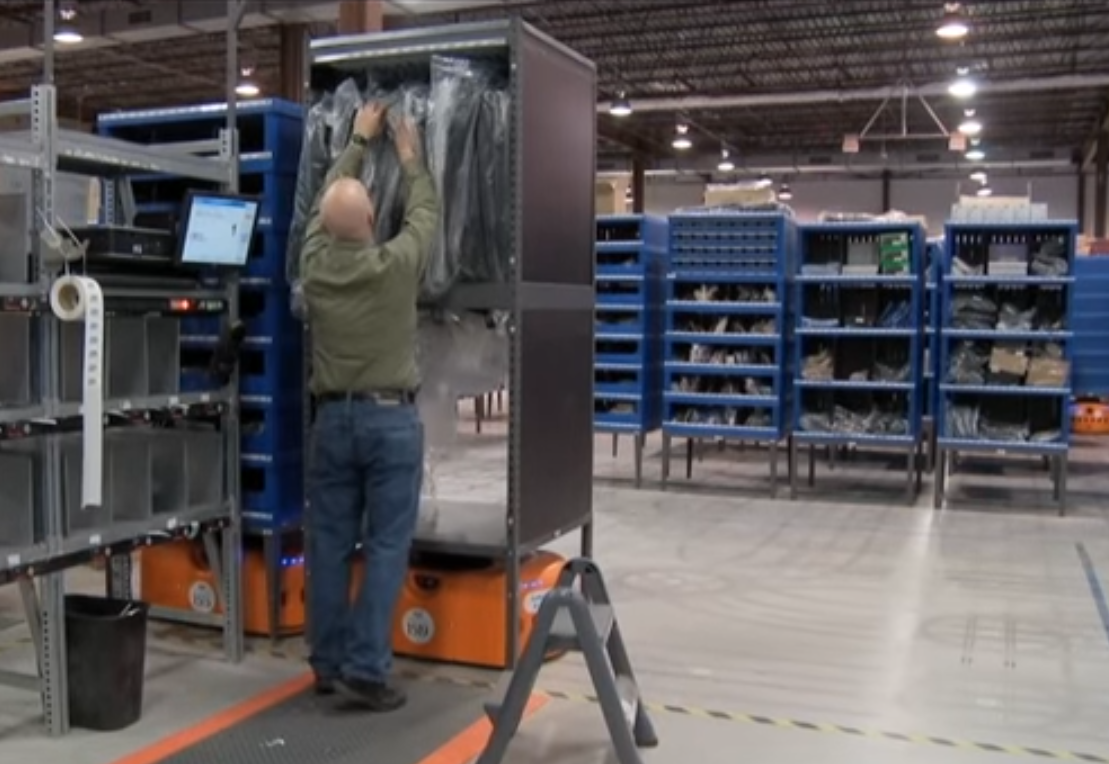
\includegraphics[width=0.6\textwidth ]{graphics/kivaprocess}
	\caption{A worker picking an order from a storage pod. The orange robot underneath is the drive unit. (\cite{kivayoutube2010quietlogistics})}
	\label{kivaprocess}
\end{figure}

%\noindent The process of order retrieval for a drive unit is as follows:
%\begin{compactenum}
%	\item Unit is told to retrieve a product
%	\item Unit moves to the storage pod containing the product and picks up the pod
%	\item Unit carries the pod to a picking station
%	\item Human worker picks the product from the pod and packs it
%	\item Unit returns the pod back to where it was picked up
%	\item Unit is told to retrieve a product
%\end{compactenum}

Kiva systems do not require a complex infrastructure to operate, a warehouse needs only storage pods, a picking station and a suitable number of drive units to operate. As long as the warehouse has space, more robots, pods or stations can be easily be added to the system to satisfy the incoming flow of customer orders. When a drive unit malfunctions it can be easily accessed and replaced. In summary, the main benefits of Kiva systems are their low initial and maintenance costs, rapidly deployment and flexibility (\cite{wurman2008coordinating}).

\subsection{Research questions}
In order to explore the improvements that can be made to improving Kiva systems, we aim to answer two main questions:

\begin{enumerate}
	\item What effect will these modifications have and how do they affect our decision when it comes to organizing the warehouse layout?
	\begin{compactitem}
		\item An optimized order process
		\item Allowing drive units are capable of maneuvering underneath storage pods
		\item An intermediate zone for drive units to drop off storage pods
	\end{compactitem}

\item How much faster will the MAPF search run by pre-computing paths and storing them in a path oracle?

\end{enumerate}

\section{Background}
\label{background}
% Description of MAPF problem, including objective function

In Kiva Systems we face a multi-agent pathfinding (MAPF) problem. MAPF aims to find a path for each agent so that they can reach their goal while ensuring that no path conflicts with another. When analyzing the performance of a MAPF solution we generally aim to reduce the makespan of the system. Specific to Kiva systems we also aim to reduce the downtime of picking stations. Outside of order picking and warehouse applications,  MAPF has usage in video games, robotics (\cite{bennewitz2002finding}), search and rescue (\cite{konolige2006centibots}) and automated ports.

% How hard is it?
Finding an optimal solution to multi-agent pathfinding is an NP-hard problem (\cite{yu2013structure}) and has found applications in systems containing a small number agents. This is not an option as Kiva systems deal with hundreds of agents, for example the Office Supply company, Staples uses 500 robots in their $30000m^{2}$ center (\cite{guizzo2008three}). The best we can get currently is a bounded suboptimal solution and this has been explored by a number of existing literature (\cite{cohen2016bounded}).

% What are the main way people solve it?
Generally methods are provided to simplify the MAPF problem, \cite{cohen2016bounded} uses user-provided highways to help guide agents towards a specific direction, greatly reducing the chance of path collisions. \cite{wilt2014spatially} identifies bottlenecks in the environment and assigns a controller to handle agents who want to pass through this area, simplifying behaviour in high collision zones. Another common technique is grouping agents into teams. \cite{ma2016optimal} splits agents into teams of 5 and presents a Conflict-Based Min-Cost-Flow algorithm which and shows that they can achieve a correct, complete and optimal solution.

% What are the main advantages and drawbacks of each approach?

%\cite{de2007design} provides a great overview of picking
Specific to order picking, it is possible to assist MAPF by manipulating incoming orders to suit the location of products. For example if a large order of one product came in, this could be interlaced with other orders, so agents do not need to all head to the same location. In a similar fashion, MAPF can be assisted by smart distribution of products across the warehouse. Take the same example where a large order of one product comes in, if the products were spread out around the warehouse this would not be an issue. This method is especially relevant in Kiva systems as storage pods can be easily moved around the warehouse by the drive units. \cite{boysen2017parts} looks at both of these aspects and found that with optimized order processing, only half the units are required to provide the supply given by a non-optimized system.

%\cite{wurman2008coordinating} provides an in depth overview of Kiva Systems, describing their benefits, usages and research areas.

%\cite{gu2010research} provides a comprehensive review of warehouse design and performance. It covers 5 major aspects, overall structure, sizing and dimensioning, department layout, equipment selection and operation strategy selection.

%\cite{de2007design} provides a survey on order picking

%\cite{strasser2015compressing} uses Compressed Path Databases.

%Unlike existing literature, in this project we aim looking at a number of other factors which are likely to simplify the pathfinding problem.

%Windowed Hierarchical Cooperative A∗. Cooperative A*. Conflict-Oriented Windowed Hierarchical Cooperative A∗. Compressed Path Databases.

\section{Methodology}
\label{Research}
\subsection{Path oracle}

Decentralised approaches are usually used in MAPF algorithms due to their lower CPU and memory requirements (\cite{wang2009bridging}) compared to a centralised approach. Decentralised MAPF involves agents independently searching for a path to their goal. Here we aim to introduce a path oracle which will pre-compute paths, removing the need for agents to perform a search at runtime. We expect to base this off the work by \cite{strasser2015compressing}, utilizing a Compressed Path Database.

Once a path is found, agents take turns following their path one step at a time until a spatio-temporal conflict occurs between agents. We choose one agent based on a user-defined utility function and this agent will continue along the path. The other agent has two options first is simply waiting until the other agent moves out of the way. The second method we may explore involves using a looking forward using a spatio-temporal reservation table to find a path without conflicts (\cite{wilt2014spatially}).

\subsection{Warehouse layout}
\label{warehouselayout}
Usually the picking station is positioned on one side of the warehouse and the pods are laid out in rows (Fig. \ref{kivalayout1}).

\begin{figure}[h]
	\centering
	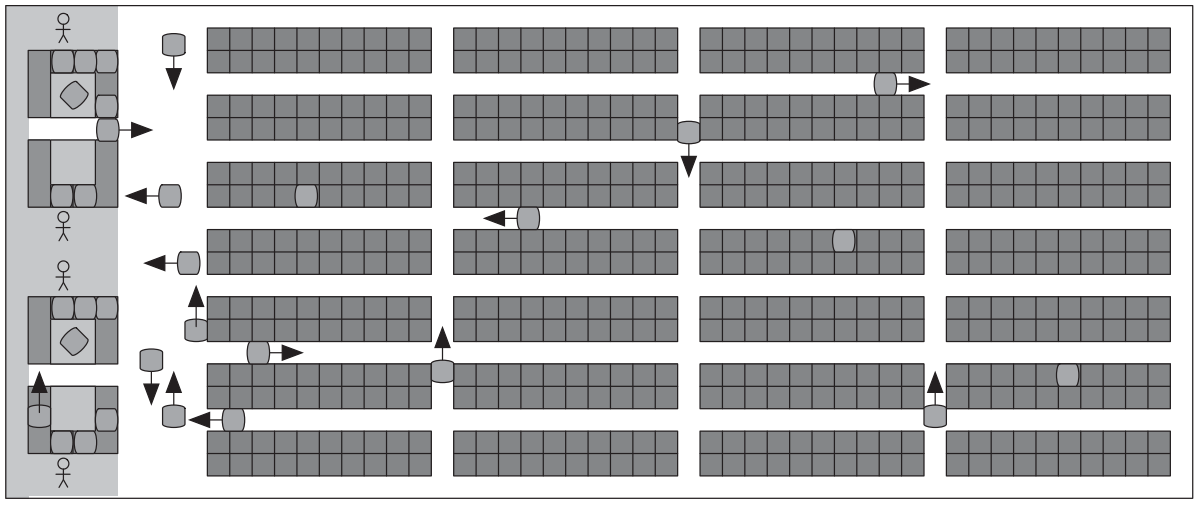
\includegraphics[width=0.9\textwidth]{graphics/kivasystemlayout}
	\caption{A Small Region of a Kiva Layout (\cite{wurman2008coordinating}). Picking stations located on the left and storage pods laid out in rows.}
	\label{kivalayout1}
\end{figure}

One of the focuses of this study is designing logical warehouse layouts, where picking stations may be distributed inbetween or around picking stations. We want to look at how this affects makespan and may help or cause issues in the MAPF. Ultimately to identify what works and what does not. A hand-made set of warehouse layouts will be the start but one possibility is the use of genetic algorithms to automatically generate a good warehouse layout.

In Section \ref{background}, we saw that \cite{wilt2014spatially} identified bottlenecks in the environment and assigned controllers to simply behaviour for any agents who wanted to travel through that zone. Inspired by this, we plan to split the warehouse into two halves and introduce an intermediate zone (See Fig \ref{kivalayout2}). Now, drive units in the far zone deliver pods to the intermediate zone instead of a pickup station. Drive units situated in the delivery zone will be responsible for retrieving pods in the intermediate zone and bringing them to pickup areas. These zones will have their own controller which handles any agents within the zone and tells agents what behaviour should occur.

\begin{figure}[h]
	\centering
	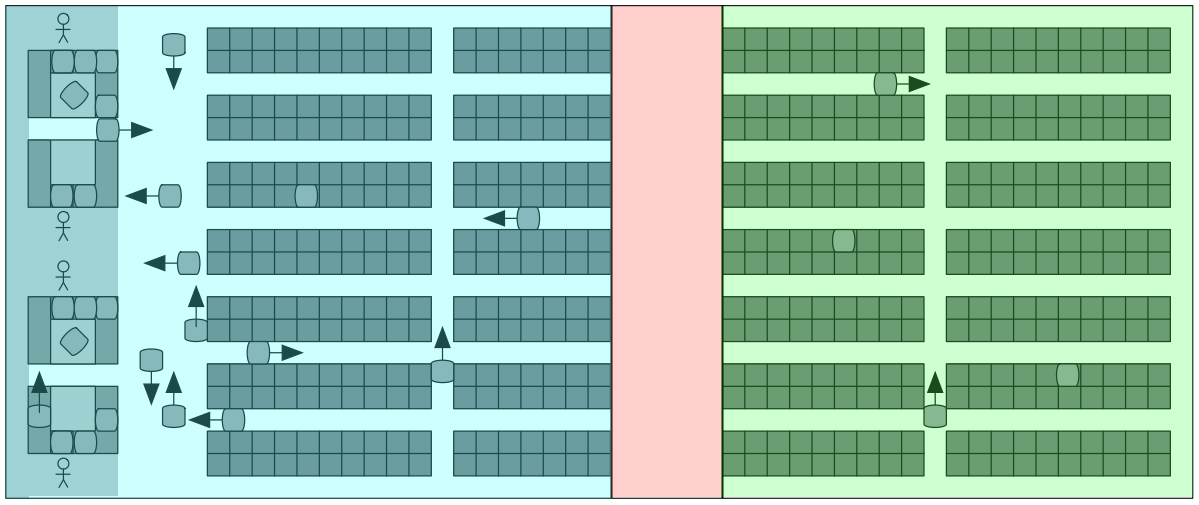
\includegraphics[width=0.9\textwidth]{graphics/kivasystemlayout_adjusted}
	\caption{Intermediate zone in red, delivery zone in blue and far zone in green}
	\label{kivalayout2}
\end{figure}

\subsection{Order processing}
\label{orderprocessing}
This process is described in detail in Section \ref{background}. Reiterating the main points of order processing we look at distribution of products around the warehouse to reduce path collisions and smart sequencing of incoming orders according to the current distribution of products around the warehouse. This is important to consider as we expect that an optimized order processing sequence will decrease the effects of having an inefficient warehouse layout. Here we may take inspiration from Robin-hood hashing.

\subsection{Capability for pathing below storage pods}
\label{beneathpods}
One of the specifications for creating a drive unit is the ability to maneuver underneath a pods to pick it up, this means that with small adjustments to the dimensions of storage pods it is possible to allow drive units to maneuver underneath the pods. Until a unit starts carrying a pod, it will not see any obstacles in the environment besides other drive units. We will explore exactly how much effect this has on reducing the makespan of the system as it will definitely reduce the number of path collisions.

\subsection{Timetable}

There are a large number of individual tasks involved in this project which have been spread across the two semesters. I have identified two major tasks which are: implementing an optimized order processing method and implementing path oracle. These have been allocated multiple weeks in semester 2 and the path oracle has been prioritized over optimized order processing as we will have implemented robin-hood hashing earlier in week 11 of semester 1. Finally, some time has been allocated to presentations or deliverables related to this project and two weeks have been allocated to focus on university examinations.

\begin{center}
{\footnotesize
\begin{tabular}{ c p{12cm} }
\multicolumn{2}{l}{\textbf{Semester 1}} \\
\hline \multicolumn{1}{c}{Week(s)} & \multicolumn{1}{c}{Plan} \\
\hline 7  & Create warehouse simulation with simple A* pathfinding \\
\hline 8-9  & Add multiple agents to the simulation using with Cooperative A* and moving between pickup stations \\
\hline 10 & Implement an order sequencer assigning generating an inflow of products to be retrieved \\
\hline 11 & Begin looking at robin-hood hashing \\
\hline 12-14 & Focus on Interim Presentation, Literature Review and Examinations \\
\hline Holidays & Look at adding an intermediate dropping zone (\ref{warehouselayout}) and implement ability to move under pods (\ref{beneathpods}) \\
\hline
\end{tabular}
}

{\footnotesize
\vspace{0.5cm}
\begin{tabular}{ c p{12cm} }
\multicolumn{2}{l}{\textbf{Semester 2}} \\
\hline \multicolumn{1}{c}{Week(s)} & \multicolumn{1}{c}{Plan} \\

\hline 7-11 & Implement Path Oracle with Compressed Path Databases \\

\hline 1-3 & Implement an optimized order processing method (\ref{orderprocessing}) \\
\hline 5-7 & Run simulation looking at combination of modifications and analyze results. Use any extra time to explore the use of genetic algorithms to generate warehouse layouts. \\
\hline 12 & Finish first draft of Final Thesis \\
\hline 13-15 & Focus on Final Presentation, Thesis and Examinations \\
\hline
\end{tabular}
}
\end{center}

\section{Expected Outcomes}
Overall we aim to contribute one major insight and one deliverable. In Section \ref{Research}, we described methods to add: an optimized order process, the capability for drive units to path under storage pods and lastly addition of an intermediate zone. What we aim to answer is how these modifications may affect our decision when it comes to designing a good warehouse layout. To showcase our results we hope to produce two main graphs comparing the makespan of the system and the idle time of picking stations across our user-defined warehouse layouts. Accompanying this would be any interesting results we see from adding or removing modifications described in Section \ref{Research}. 

For our deliverable, we hope to produce an improved MAPF solution utilizing a pre-computed path oracle and a simulation showcasing its usage in a simulated Kiva system. Similarly, we will showcase the results by comparing the makespan of the system and idle time of picking stations to alternative MAPF techniques.

\bibliographystyle{dcu}
\bibliography{bibliography}

\end{document}
